% !TeX root = ../defense.tex
\section{Steady Flow Aerodynamic Model}
\frame{\sectionpage}
\begin{frame} 
For an ideal polytropic gas with density, $\rho$, velocity, $\vec{V}$, and 
pressure, $p$ , the Euler equations are,
\begin{align}
    \frac{D\rho}{Dt} = - \rho \nabla \cdot \vec{V} 
    \label{eqn:CompressibleConservationOfMass} \\
    \frac{D\vec{V}}{Dt} = - \frac{\nabla p}{\rho} + \vec{g} 
    \label{eqn:CompressibleConservationOfMomentum} \\
    \frac{Dp}{Dt} = - \gamma p \nabla \cdot \vec{V} 
    \label{eqn:CompressibleConservationOfEnergy} \\
\end{align}
where Equations (\ref{eqn:CompressibleConservationOfMass},
\ref{eqn:CompressibleConservationOfMomentum},
\ref{eqn:CompressibleConservationOfEnergy}) are the conservation of mass, 
momentum, and energy equations respectively. 
\end{frame}
\begin{frame}
If the flow is assumed to be asymmetric, then the radial velocity component is 
zero. With this considered, the velocity vector ,$\vec{V}$ in cylindrical coordinates 
become,
\begin{align}
    \vec{V}(r,\theta,x) &= v_x(r) \hat{e}_x + v_{\theta} (r) \hat{e}_{\theta} 
    \label{eqn:VelocityVector}
\end{align}
  
where $\hat{e}_x$ and $\hat{e}_{\theta}$ are unit vectors for the axial and 
tangential directions.The gradient operator ,$\nabla$ in cylindrical
coordinates, is 

\begin{align}
	\vec{\nabla} 
	&= \hat{e}_r \frac{\partial} {\partial r} + 
	\frac{1}{r} \hat{e}_{\theta}   
	\frac{\partial} {\partial \theta} + 
	\frac{\partial }{\partial z} \hat{e}_z = 0
    \label{eqn:NablaInCylindrical}
\end{align}


    
\end{frame}
\begin{frame}
For a steady flow, ($\partial/\partial t = 0$) , the compressible flow equations
can be further reduced to,

\begin{align}
    \nabla (\vec{V} \rho) &=  0 \\
    (\vec{V}\cdot \nabla) \vec{V} &=  0\\
    \nabla S &= 0
\end{align}

where $S$ represents the entropy in the mean flow.


\end{frame}
\begin{frame}{Nonuniformities from swirling mean flow}
    

If the mean flow contains a swirling component, i.e. a velocity vector in the 
tangential direction, the mean quantities, pressure , density are non-uniform, 
thus also changing the speed of sound. By integrating the radial momentum
equation, an expression for the speed of sound was established to account for 
the resulting nonuniformities due to rotations in the flow. 
\begin{equation}
    p = \int_{r_{min}}^{r_{max}} \frac{\rho v_{\theta}^2}{r} dr 
    \label{eqn:radialmomentum_integrated}
\end{equation}

where $r_{min}$ and $r_{max}$ are the bounds of the radius. Since the flow
is isentropic, the pressure is related to the speed of sound through $\nabla p =
A^2 \nabla \rho$; which is used to compute $\rho$. 

\end{frame}
\begin{frame}

With the relationship 
$A^2 = \kappa p/\rho$, the speed of sound is found to be,

    
\begin{align*}
\tilde{A}(\tilde{r}) &= exp\left[\left(\frac{1 - \gamma}{2}\right)\int_{\tilde{r}}^{1}\frac{M_{\theta}}{\tilde{r}}{\partial \tilde{r}}\right]	
\end{align*}

\end{frame}
\begin{frame}

    
\end{frame}
\section{Unsteady Flow Aerodynamic Model}
\frame{\sectionpage}
\begin{frame}
    
Goldstein demonstrated the linearized momentum and continuity PDE  can be 
combined to derive the convective wave equation by taking the divergence of
the momentum equation and taking the difference of the substantial derivative
of the conservation of mass equation to yield,

\begin{equation}
    \frac{1}{A^2}\frac{D^2\tilde{p}}{Dt^2} -
    \nabla^2 \tilde{p} =
    2 \bar{\rho} \frac{d V_x}{d x} \frac{\partial  \tilde{v}_r}{ \partial x} 
    \label{eqn:KousensWaveEquation}
\end{equation}

\end{frame}
\begin{frame}
    

In the case of sheared flow, $dV_x/dx = 0$ the right hand side will be zero 



\begin{align*}
    \frac{1}{A^2}\left(
        \frac{\partial^2 \tilde{p}}{\partial t^2} + 
        \vec{V}\cdot \vec {\nabla} (\tilde{p}) 
    \right) -
    \nabla^2
    \tilde{p} &=
    0 \\
\end{align*}

\end{frame}
\begin{frame}

Utilizing the relation, $\tilde{p} = p/\bar{\rho} A^2$,substituting the 
definitions for $\nabla$ and $\nabla^2$ and setting $\vec{V} =0$
in cylindrical coordinates gives,



\begin{align*} 
    \frac{1}{A^2}\left(
        \frac{\partial^2 {p}}{\partial t^2}
    \right) - 
        \left(
            \frac{\partial^2 {p}}{\partial t^2} + 
            \frac{1}{\tilde{r}}\frac{\partial p}{\partial r} +
            \frac{1}{\tilde{r}^2} \frac{\partial^2 p}{\partial \theta^2} + 
            \frac{\partial^2 p}{\partial x^2} 
        \right) &= 0  
\end{align*} 

    
\end{frame}
\begin{frame}
    

 The method of separation of variables requires an assumed solution as well as initial and boundary 
conditions. 

For a partial differential equation, the assumed solution can be a 
linear combination of solutions to a system of ordinary differential equations that
comprises the partial differential equation. 

Since $p$ is a function of four variables, the solution is 
assumed to be a linear combination of four solutions.

Each solution is assumed to be Euler's identity, a common ansant for linear partial 
differential equations and boundary conditions.

 Defining,

\begin{equation}
    p(x,r,\theta,t) = X(x) R(r) \Theta(\theta) T(t)
\end{equation}
\end{frame}
\begin{frame}
where, 

\begin{align*}
    X(x) &=
    A_1 e^{ik_x x} +
    B_1 e^{-ik_x x }\\
    \Theta(\theta) &=
    A_2 e^{i k_{\theta} \theta } +
    B_2 e^{-ik_{\theta} \theta }\\
    T(t) &=
    A_3 e^{i \omega t } +
    B_3 e^{-i\omega t  }
\end{align*}



The next step is to rewrite the wave equation in terms of $X$, $R$, $\Theta$,
and $T$. To further simplify the result, each term is divided by $p$.

\begin{equation}
    \frac{1}{A^2} \frac{1}{T}\frac{\partial^2 T}{\partial t^2} = 
    \frac{1}{R}\frac{\partial^2 R}{\partial r^2 } +
    \frac{1}{r}\frac{1}{R}\frac{\partial R}{\partial r}  + 
    \frac{1}{r^2}\frac{1}{\Theta}\frac{\partial \Theta}{\partial \theta} + 
    \frac{1}{X}\frac{\partial^2 X}{\partial x^2}
    \label{eqn:waveode}
\end{equation}
\end{frame}
    

\begin{frame}
    

\begin{equation}
    \frac{1}{R}
    \left(      
    \frac{\partial^2 R}{\partial r^2 } +
    \frac{1}{r}\frac{\partial R}{\partial r}  
\right) -
    \frac{k_{\theta}^2}{r^2}-  
    k_x^2 + k^2 = 0
    \label{eqn:waveode3}
\end{equation}
The remaining terms are manipulated to follow the same form as \textit{Bessel's Differntial 
Equation} ,

\begin{equation}
    x^2 \frac{d^2 y}{dx^2} + x \frac{dy }{dx } + (x^2 - n^2) y = 0
    \label{eqn:besselODE}
\end{equation}

The general solution to Bessel's differential equation is a linear combination of
the Bessel functions of the first kind, $J_n(k_r r)$ and of the second kind, $Y_n(k_r r)$ 
\cite{wolphram:bessel}. The subscript $n$ refers to the order of Bessel's equation.
    
\begin{equation}
    R(r) = (AJ_n(k_r r) + BY_n(k_r r)) 
    \label{eqn:besselsolution}
\end{equation}
where the coefficients $A$ and $B$ are found after applying radial
boundary conditions. %and there is an exponential dependence. 
\end{frame}
\begin{frame}
By rearranging Equation (\ref{eqn:waveode3}), a comparison can be made to Equation
(\ref{eqn:besselODE}) to show that the two equations are of the same form. 

The first step is to revisit the radial derivatives that have not been addressed.
As was done for the other derivative terms, the radial derivatives will also 
be set equal to a separation constant, $-k_r^2$. 

\begin{align}
    \underbrace{\frac{1}{R}
    \left(      
    \frac{\partial^2 R}{\partial r^2 } +
    \frac{1}{r}\frac{\partial R}{\partial r}  
\right) -
    \frac{k_{\theta}^2}{r^2}}_{-k_r^2}-  
    k_x^2 + k^2 = 0
    \label{eqn:wavenumber_without_kr}
\end{align}

\end{frame}
\begin{frame}
    

The reader may be curious as to why the tangential separation constant $k_{\theta}$ is 
included within the definition of the radial separation constant. 

Recall the ODE for the tangential direction, 

\begin{align*}
    \frac{\partial \Theta}{\partial \theta} \frac{1}{\Theta} = - k_{\theta}^2\\
    \frac{\partial \Theta}{\partial \theta} \frac{1}{\Theta} + \Theta k_{\theta}^2 = 0 
\end{align*}

where the solution is more or less,

\begin{align*}
    \Theta(\theta) = e^{i k_{\theta} \theta}
\end{align*}

In order to have non trivial, sensible solutions, the value of $\Theta(0)$ and
$\Theta(2\pi)$ need to be the same, and this needs to be true for any multiple 
of $2\pi$ for a fixed r. Taking $\Theta$ to be one, a unit circle, it can be shown that the domain
is only going to be an integer multiple. Therefore, there is an implied periodic
azimuthal boundary condition, i.e. $0<\theta\leq 2 \pi$ and $k_{\theta}=m$. 

\end{frame}

\begin{frame}
There is a unique treatment for the radial derivatives.


\begin{align*}
    -k_r^2 =\frac{1}{R}
    \left(      
    \frac{\partial^2 R}{\partial r^2 } +
    \frac{1}{r}\frac{\partial R}{\partial r}  
\right) -
    \frac{m^2}{r^2} 
\end{align*}
To further simplify, the chain rule is used to do a change of variables, $x = k_r r$
\begin{align*}
    \frac{\partial R}{\partial r} &= \frac{dR}{dx}\frac{dx}{dr}\\
    &=
    \frac{dR}{dx}\frac{d}{dr}\left( k_r r \right) \\
    &=
    \frac{dR}{dx} k_r 
\end{align*} 


    
\end{frame}
\begin{frame}
    
\begin{align*}
    \frac{\partial^2 R}{\partial r^2} &= \frac{d^2R}{dx^2}\left(\frac{dx}{dr}\right)^2 + 
    \frac{dR}{dr}\frac{d^2x}{dr^2}\\
    &=
    \frac{d^2R}{dx^2}\frac{d}{dr} k_r^2 + k_r \frac{d^2r}{dr^2}\\
    &=
    \frac{d^2R}{dx^2}\frac{d}{dr} k_r^2
\end{align*} 

Substituting this into Equation (\ref{eqn:waveode3}),
\begin{equation}
    \left(\frac{d^2R}{dx^2}k_r^2 +
    \frac{1}{r}\frac{d^2R}{dx^2}k_r\right) +
    \left(k_r^2 - \frac{m^2}{r^2}\right)R
    \label{eqn:waveode4}
\end{equation}
Dividing Equation \ref{eqn:waveode4} by $k_r^2$,

\end{frame}
\begin{frame}
\begin{equation}
    \left(\frac{d^2R}{dx^2} +
    \frac{1}{k_r r}\frac{d^2R}{dx^2}\right) +
    \left(1  - \frac{m^2}{k_r^2 r^2}\right)R
    \label{eqn:waveode5}
\end{equation}

\begin{equation}
    \left(\frac{d^2R}{dx^2} +
    \frac{1}{x^2}\frac{d^2R}{dx^2}\right) +
    \left(1  - \frac{m^2}{x^2}\right)R
    \label{eqn:waveode6}
\end{equation}
\end{frame}
\begin{frame}
    
Multiplying Equation (\ref{eqn:waveode6}) by $x^2$ gives,

\begin{equation}
    \frac{d^2R}{dr^2}x^2 + 
    \frac{dR}{dr}x + 
    \left( x^2 - m^2 \right)R
    \label{eqn:finalradialode}
\end{equation}
which matches the form of Bessel's equation
\end{frame}
\begin{frame}

Therefore, the solution goes from this,
to this,


\begin{equation}
    y(x) = AJ_n(x) + BY_n(x)
    \label{eqn:besselsolution}
\end{equation}
to this,

\begin{equation}
    R(r) = AJ_n(k_r r) + BY_n(k_r r)
    \label{eqn:besselsolution}
\end{equation}
\end{frame}
\begin{frame}
    
\subsubsection{Hard Wall boundary condition}
\begin{align*}
    \frac{\partial p}{\partial r}|_{r = r_{min}}  =\frac{\partial p}{\partial r}|_{r = r_{max}} = 0 \rightarrow 
    \frac{\partial}{\partial r} \left( X\Theta T R \right) &= 0 \\
    X \Theta T\frac{\partial R}{\partial r}  &= 0 \\
    \frac{\partial R}{\partial r}  &= 0 
\end{align*}

where,


\begin{align*} 
    \frac{ \partial R}{\partial r}|_{r_{min}} &= AJ_n'(k_r r_{min}) + B Y_n' (k_r r_{min}) = 0 
    \rightarrow B = -A \frac{J_n'(k_r r_{min})}{Y_n'(k_r r_{min})}
\end{align*}

\end{frame}
\begin{frame}
\begin{align*} 
    \frac{ \partial R}{\partial r} &= AJ_n'(k_r r_{max}) + B Y_n' (k_r r_{max}) = 0 \\
                                   &= AJ_n'(k_r r_{max}) - A\frac{J_n' (k_r r_{min})}{Y_n'(k_r r_{min})} Y_n' (k_r r_{max}) = 0 \\
                                   &= \frac{J_n'(k_r r_{min})}{J_n' (k_r r_{max})} - \frac{Y_n'(k_r r_{min})}{Y_n' (k_r r_{max})} = 0 
\end{align*}
where $k_r r$ are the zero crossings for the derivatives of the Bessel functions of the first and second kind.

In summary, the wave equation for no flow in a hollow duct with hard walls is obtained 
from Equation (\ref{eqn:wavenumber_without_kr}).
\begin{equation}
    k^2 = k_r^2 + k_x^2
    \label{eqn:wavenumber_equation}
\end{equation}

\end{frame}
% \section{Results Update}
% \frame{\sectionpage}

% \begin{frame}{Motivation}
%     \begin{alertblock}{How is the analytical solution computed for Sound Prop. in Uniform Axial Flow}
%     \begin{enumerate}[<+->]\itemsep9pt
%         \item The analytical solution are the axial wavenumbers and propagating
%             modes for a given frequency, axial velocity and azimuthal mode order.
%         \item For a given azimuthal mode, there is a range of radial modes.
%         \item These radial modes can be categorized based on the sign of the axial wavenumber and if it is
%             complex in value. 
%         \item Propagating modes are defined by axial wavenumbers, $k_x$, that have a real-part only, yielding 
%             the assumed fluctuation to resemble Euler's Formula ($e^{ik_x x}$). 
%         \item On the other hand, if the $k_x$ is complex, then the mode will resemble an exponentially decaying
%             function since the imaginary number cancels, leaving a minus sign in front of
%             the axial wavenumber.
%     \end{enumerate}
%     \end{alertblock}

%     \tiny
%     % \hspace{3.75em}\url{http://www.klimaschutzplan2050.de/en/action-areas/energy-sector/}
% \end{frame}
% \begin{frame}

% \begin{equation}
%     k_x  = \frac{- M_x k \pm \sqrt{k^2 - ( 1 - M_x^2) J_{m,n}'^2 }}{\left( 1 - M_x^2 \right)}.
%     \label{eqn:ax_wavenumb}
% \end{equation}

% where $M_x$ is the axial Mach number, $k$ is the temporal (referred to as reduced)
% frequency, and $J_{m,n}'$ is the derivative of the Bessel function of the first kind.  
% The $\pm$ accounts for both upstream and downstream modes.

% The condition for propagation is such that the axial wavenumber is larger than 
% a ``cut-off'' value

% \begin{equation}
%     k_{x,real}  = \frac{\pm M_x k }{\left( M_x^2 - 1 \right)}.
%     \label{eqn:cuton}
% \end{equation}


% \end{frame}
% \begin{frame}
    
% Every term that is being raised to the one half i.e. square rooted must 
% be larger than zero to keep axial wavenumber from being imaginary. The mode 
% will propagate or decay based on this condition. Recall thaT the mode is of the 
% form 
% \begin{equation}
%     e^{i k_x x}
%     \label{eqn:fluctuationexample}
% \end{equation}
% if $k_x$ has a real part, $k_{x,real}$ and an imaginary part $i k_{x,imag}$ 
% then,

% \begin{align}
%     &= e^{i k_x x} \\
%     &= e^{i (k_{x,real}+ i k_{x,imag}) x} \\
%     &= \underbrace{e^{i k_{x,real}x}}_{\textit{amplitude}} \underbrace{e^{- k_{x,imag} x}}_{\textit{exponential decay}} 
% \end{align}


% \end{frame}
% \begin{frame}
    

% Although the ``cut-off'' decay to nearly zero rapidly, the rate at which this occured
% was not much of a concern earlier on in turbomachinery design. As nacelles 
% continue to grow shorter, a mode that is ``cut-off'' may make it outside the duct.

% For this work a desired amplitude was arbitrarily chosen for a mode, $y_{desired}$
% and then the axial location at which this occurred, $x_{desired}$ which 
% can be compared against a desired length for a nacelle.  
% Since SWIRL assumes an infinitely long duct, there is nothing limiting the 
% modes propagation with respect to nacelle length. For example, if the 
% desired amplitude is one percent, then $x_{desired}$,

% \begin{align*}
%     0.01 &=  e^{-10 x_{desired}},\\
%     -\frac{ln|0.01|}{10} &=  x_{desired},\\
%     -\frac{ln|0.01|}{10} &= 0.4605170185988091 .
% \end{align*}

% \end{frame}
% \begin{frame}
    


%  \begin{figure}
%      \centering
%      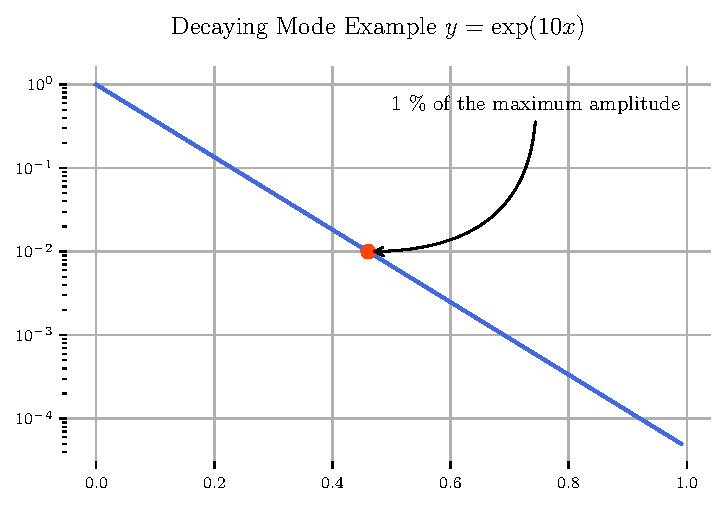
\includegraphics[width=0.7\textwidth]{/home/jeff-severino/SWIRL/CodeRun/04-plotReport/tex-outputs/desired_cut_off_location_1_percent_of_max2.pdf}
%      \caption{Decaying mode with $k_x = 0 + 10j$ and unit amplitude. One percent
%      of the maximum amplitude is identified for nacelle length comparison}
%      \label{fig:decaying_mode_with_1_percent_amp}
%  \end{figure}
 
 
% In general,
% \begin{align*}
%     y_{desired} &=  e^{-k_{x,imag} x_{desired} }\\
%     -\frac{ln|y_{desired}|}{k_{x,imag}} &=  x_{desired}
% \end{align*}
% \end{frame}
% \begin{frame}
% \section{Analytical Test Case 1}
% \begin{table}[h!]
%     \centering
%     \begin{tabular}{|l|l|}
%         \hline
%         $\sigma$ & \textit{0.0} \\ \hline
%         $k$      & \textit{10}   \\ \hline
%         $m$      & \textit{2}    \\ \hline
%         $M_x$    & \textit{0.3}  \\ \hline
%     \end{tabular}
%     \caption{Validation test case parameters, Uniform Flow Annular Duct} 
% \end{table}

% \end{frame}

% \begin{frame}
    
%  \begin{figure}
%      \centering
%      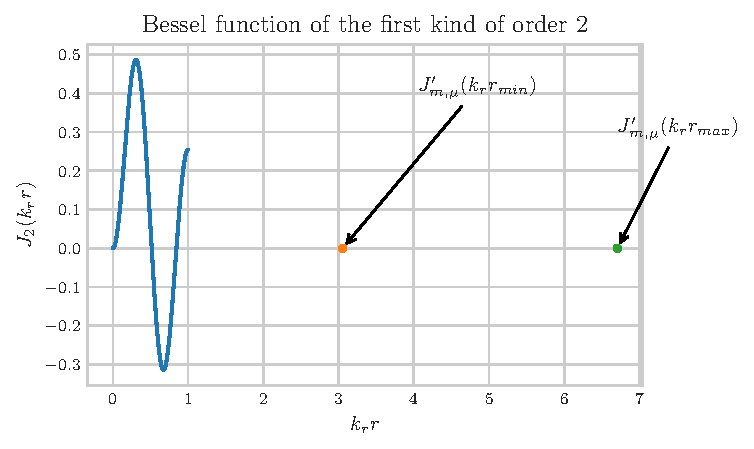
\includegraphics[width=0.7\textwidth]{/home/jeff-severino/SWIRL/CodeRun/04-plotReport/tex-outputs/bessel_analytical_test_case.pdf}
%      \caption{The Bessel function with the values of $J'_{m,\mu}$ labeled}
%      \label{fig:decaying_mode_with_1_percent_amp}
%  \end{figure}
% \end{frame}



% \begin{frame}
    
%  \begin{figure}
%      \centering
%      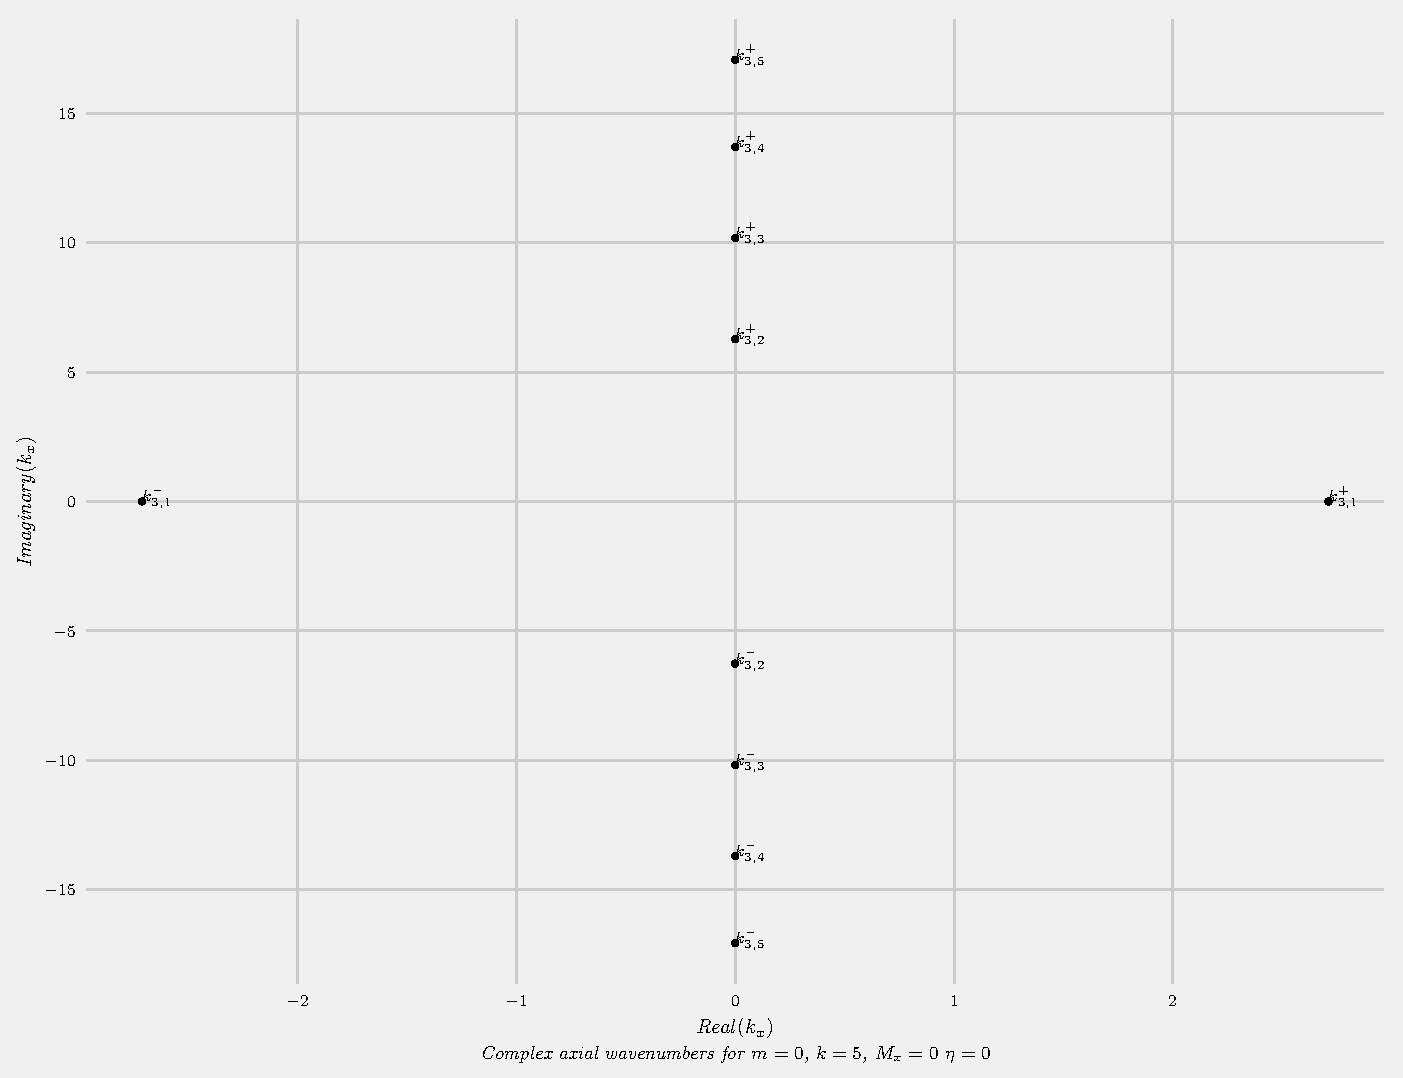
\includegraphics[width=0.7\textwidth]{/home/jeff-severino/SWIRL/CodeRun/04-plotReport/tex-outputs/axial_wavenumber_analytical_test_case.pdf}
%      \caption{The Bessel function with the values of $J'_{m,\mu}$ labeled}
%      \label{fig:decaying_mode_with_1_percent_amp}
%  \end{figure}
% \end{frame}


% \begin{frame}{Normalized Mode}

    
%  \begin{figure}
%      \centering
%      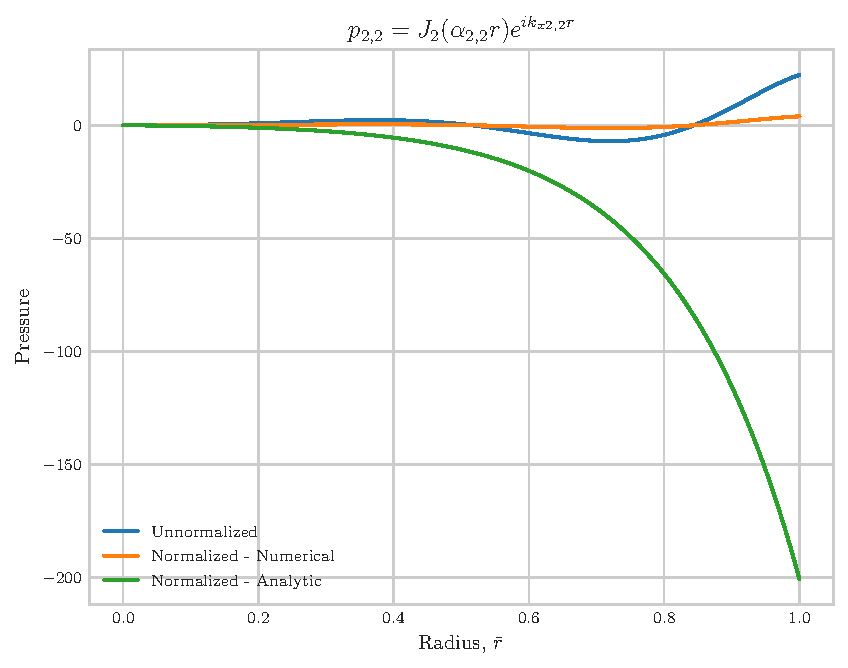
\includegraphics[width=0.7\textwidth]{/home/jeff-severino/SWIRL/CodeRun/04-plotReport/tex-outputs/Normalized_Mode_test_case.pdf}
%      \caption{The Bessel function with the values of $J'_{m,\mu}$ labeled}
%      \label{fig:decaying_mode_with_1_percent_amp}
%  \end{figure}
% \end{frame}
% \begin{frame}
    
% \end{frame}




% \begin{frame}{Future Work}
%     \begin{alertblock}{}
%     \begin{enumerate}[<+->]\itemsep9pt
%         \item I need to use sanity checks to ensure that the normalization provided
%             by Rienstra is implemented correctly.
%         \item While the numerical normalized mode has an integral of one, the 
%             analytical mode is not.
%         \item a few things that have been checked along the way but need to be 
%             reported are,
%         \item Zero's of $J'_m$ 
%         \item Value of $J_m$ at the zero location
%         \item Relations involving integrals If it so not too cumbersome.
%             There are some simplifications that could be checked\ldots 
%         \item Check the analytical test case that has been reported in literature.
%            The difference is that $\sigma = 0.25$
%     \end{enumerate}
%     \end{alertblock}

%     \tiny
%     % \hspace{3.75em}\url{http://www.klimaschutzplan2050.de/en/action-areas/energy-sector/}
% \end{frame}

% % \begin{frame}{Perspective}{Disciplines for investigating energy topics}
% %     \begin{center}
% %     \begin{tikzpicture}[
% %       node distance=4.5em and .75cm,font=\small
% %     ]
% %     % flowboxes
% %     \node[flowbox] (physik) {
% %         \fbtitle{Physics}\vphantom{yÖ}
% %     \nodepart{two}
% %         \begin{minipage}{.16\textwidth}
% %             \centering
% %             Theoretical\\ feasibility\\
% %             \scriptsize (Natural laws)
% %         \end{minipage}
% %     };

% %     \node[flowbox,right=of physik] (technik) {
% %         \fbtitle{Engineering}\vphantom{yÖ}
% %     \nodepart{two}
% %         \begin{minipage}{.16\textwidth}
% %             \centering
% %             Technical\\ feasibility\\
% %             \scriptsize (Technologies)
% %         \end{minipage}
% %     };

% %     \node[flowbox,right=of technik] (econ) {
% %         \fbtitle{Economy}\vphantom{yÖ}
% %     \nodepart{two}
% %         \begin{minipage}{.16\textwidth}
% %             \centering
% %             Economic\\ feasibility\\
% %             \scriptsize (Funding)
% %         \end{minipage}
% %     };

% %     \node[flowbox,right=of econ] (society) {
% %         \fbtitle{Society}\vphantom{yÖ}
% %     \nodepart{two}
% %         \begin{minipage}{.16\textwidth}
% %             \centering
% %             Social\\ feasibility\\
% %             \scriptsize (Decision space)
% %         \end{minipage}
% %     };

% %     \uncover<2->{%
% %         \draw [decorate,decoration={brace,amplitude=10pt,mirror},ultra thick,jdblue]
% %             ($(technik.south west) + (-.2em,-1em)$) --
% %             ($(econ.south east)    + (+.2em,-1em)$) coordinate[midway,yshift=-3.8em] (midpoint-below);
    
% %         \node[flowbox] at (midpoint-below) (tech-econ)  {
% %             \fbtitle{Techno-economic modelling}\vphantom{yÖ}
% %         \nodepart{two}
% %             \begin{minipage}{.4\textwidth}
% %                 \centering
% %                 How much energy?
% %                 For how much?\vphantom{yÖ}
% %             \end{minipage}
% %         };
% %     }
% %     \end{tikzpicture}
% %     \end{center}
% % \end{frame}
